% no notes
\documentclass{beamer}
% notes and slides
% \documentclass[notes]{beamer}
% notes only
% \documentclass[notes=only]{beamer}

\usetheme{metropolis}           % Use metropolis theme
%\setbeamertemplate{caption}[default]
\usepackage{booktabs} % Allows the use of \toprule, \midrule and \bottomrule in tables
\usepackage[scale=2]{ccicons}

\usepackage{graphicx} % Allows including images
\usepackage{multirow}
\usepackage{tikz}
%usepackage{circuitikz}
\usepackage{url}
\usepackage{pgfplots}
\pgfplotsset{compat=newest}
\usepgfplotslibrary{groupplots,dateplot}
\usetikzlibrary{patterns,shapes.arrows}
\usepackage{standalone}
\usepackage{adjustbox}
\usepackage{lmodern,textcomp}
\usepackage{pgfplots}
\usepackage{amsmath}
\usepackage{amssymb}
\usepackage{eurosym}
\usepackage{amsthm}
\usepackage{multimedia}
\usepackage{standalone}
\usepackage{csquotes}
\usepackage{standalone}
%\usepackage{fontspec}
%\usepackage{unicode-math}


\PassOptionsToPackage{american}{babel} % change this to your language(s), main language last
% Spanish languages need extra options in order to work with this template
% \PassOptionsToPackage{spanish,es-lcroman}{babel}
\usepackage{babel}

\PassOptionsToPackage{%
  backend=biber,bibencoding=utf8, %instead of bibtex
  %backend=bibtex8,bibencoding=ascii,%
  language=auto,%
  style=numeric-comp,%
  %style=authoryear-comp, % Author 1999, 2010
  %bibstyle=authoryear,dashed=false, % dashed: substitute rep. author with ---
  style=alphabetic,
  sorting=nyt, % name, year, title
  maxbibnames=10, % default: 3, et al.
  %backref=true,%
  %natbib=true % natbib compatibility mode (\citep and \citet still work)
}{biblatex}
\usepackage{biblatex}

\addbibresource{bib.bib}


\title{Statistics for Machine Learning}
\date{\today}
\institute{High-Performance Computing and Analytics Lab, University of Bonn}
\author{Moritz Wolter}

\titlegraphic{
\includegraphics[width=2.00cm]{UNI_Bonn_Logo_Standard_RZ.pdf}}
\begin{document}
    \maketitle

    \begin{frame}
    \frametitle{Overview} 
    \tableofcontents

    \end{frame}


    \begin{frame}{Why statistics?}
      \begin{itemize}
        \item Its useful and can help us make decisions when outcomes are uncertain.
        \item Like getting a vaccination.
        \item Statistics is also an integral part of machine learning. Without it, we won't
         understand many machine learning methods.
        \item Neural networks, for example, model class probabilities in the classification case.
      \end{itemize}
      Today's talk is mostly based on \cite{haslwanter2016introduction},
      \cite{deisenroth2020mathematics} and some \cite{unpingco2016python}.
    \end{frame}

    \section{Foundational Statistical Concepts}
    \begin{frame}{Foundational Statistical Concepts}
      \begin{figure}
        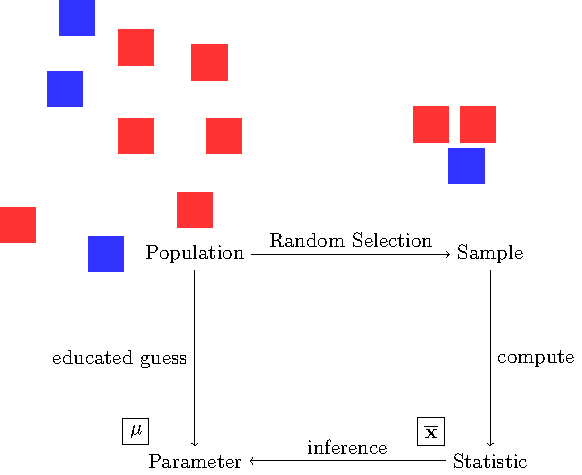
\includegraphics[width=0.75\linewidth]{./figures/intro.pdf}
        \caption{Statistical inference means inferring something about a population using information from
                 samples \cite{haslwanter2016introduction}.}
      \end{figure}
      \note{
        Population includes all of the elements from a set of data.
        Sample consists of one or more observations from the population. \\

        Parameter Characteristic of a distribution describing a population, such as the
        mean or standard deviation of a normal distribution. Often notated using Greek
        letters. \\

        Statistics: A numerical value that represents a property of a random sample. 
        Examples of statistics are \\
        - the mean value of the sample data. \\
        - the range of the sample data. \\
        - deviation of the data from the sample mean. \\
      
      Machine learning and statistics are both concerned with the construction of
      models to explain data. In statistics data is observed and we try to figure
      out a process that explains the data. In machine learning we look for a best-fit
      \cite{deisenroth2020mathematics}.
    }
    \end{frame}

    \begin{frame}{Probability and random variables \cite{deisenroth2020mathematics}}
      \begin{block}{Sample space $~\Omega $}
        The samples space contains all possible outcomes of an experiment.
        A coin toss, for example, can have two outcomes heads (h) or tails (t).
        Which leads to the set $\{h, t \}$. Two sucessive tosses generate the
        larger space $\{ hh, tt, ht, th \}$. 
      \end{block}
      \begin{block}{Event space $~\mathcal{A}$}
        A set of events, an event is a set of outcomes from the sample space.
      \end{block}
      \begin{block}{Probability $P$}
        With each event $\mathcal{A}$ we associate a number P($\mathcal{A}$).
        This number measures the probability that the event will occur.
      \end{block}
      \note{
        Lets consider a hypothetical bag. The bag contains dollar $\$$ and euro $\mbox{\euro}$ coins.
        Of ten coins in the bag four are euro coins. If we draw twice the probability
        space will be the set $\{ $\mbox{\euro}$\mbox{\euro}, \$$\mbox{\euro}, $\mbox{\euro}\$, \$\$ \}$. 
        We can now construct a discrete function for the random variable $X$.
        $X(\mbox{\euro},\mbox{\euro}) = 2$, $X(\mbox{\euro}, \$) = 1$, $X(\$, \mbox{\euro}) = 1$,
        $X(\$,\$) = 0$ 
        
        \begin{align}
        P(X = 2) &= P((\mbox{\euro}, \mbox{\euro})) = P(\mbox{\euro}) \cdot P(\mbox{\euro}) = 0.4 \cdot 0.4 &= 0.16 \\
        P(X = 1) &= P((\mbox{\euro}, \$) \cup P((\$, \mbox{\euro})) = P((\mbox{\euro}, \$) + P((\$, \mbox{\euro}))  \nonumber \\
                 &= 0.4 \cdot (1 - 0.4) + (1 - 0.4) \cdot 0.4 &= 0.48 \\
        P(X = 0) &= P(\$) \cdot P(\$) = 0.6 \cdot 0.6 &= 0.36 
        \end{align}
      }
    \end{frame}
    

    \begin{frame}{Towards distribution functions \cite{haslwanter2016introduction}}
      \begin{block}{Random Variable}
        $\;$ \\
        A random variable $X$ is an uncertain quantity. Its value depends on random events.
        A good example is the result of a dice roll.
      \end{block}

      \begin{block}{Probability Distribution}
        $\;$ \\
        Probability density functions are a mathematical tool to describe the randomness of data
        in populations and samples.
      \end{block}

    \end{frame}

    \begin{frame}{Discrete probabilities \cite{deisenroth2020mathematics}}
      We can think about probabilities for multiple discrete random variables,
      by filling out multidimensional arrays or tables.
      Our arrays contain probability numbers. For two variables,
      \begin{align}
        P(X = x_i, Y = y_i) = \frac{n_{ij}}{N}
      \end{align}
      above $n_{ij}$ counts the events for each corresponding event $x_i$, $y_i$. And
      $N$ measures all events in total.
      \begin{table}
      \centering
      \begin{tabular}{c c | c | c | c | c | c | c} %\cline{2-6} \rotatebox{90}{$\rbrace$}
          &       \multicolumn{6}{c}{$\;  \;  \; \; c_i$}     &   \\ 
          &       \multicolumn{6}{c}{$\;  \; \; \;$ \rotatebox{90}{$\rbrace$}}  &       \\ \cline{3-7}
          & $y_1$ &  $\;$ & $\;$  &  $\;$   & $\;$&  $\;$ & $\;$   \\ \cline{3-7} 
      Y   & $y_2$ &  $\;$ & $\;$  & $n_{ij}$& $\;$&  $\;$ & $ \rbrace r_j$ \\ \cline{3-7}
          & $y_3$ &  $\;$ & $\;$  & $\;$    & $\;$&  $\;$ & $\;$  \\ \cline{3-7}
          %&       & $x_1$ & $x_2$ & $x_3$ & $x_4$ & $x_5$ &       \\
          & \multicolumn{6}{c}{$\;$ $\;$ $\;$ $x_1$ $x_2$ $\;$ $x_3$ $\;$ $x_4$ $\;$ $x_5$} & \\
          &        \multicolumn{6}{c}{X}       &       \\
      \end{tabular}
    \end{table}
  \end{frame}

  \begin{frame}{Marginal and conditional probability}
    We can compute marginal probabilities by summing rows or columns.
    \begin{align}
      P(X = x_i) = \frac{c_i}{N} = \frac{ \sum_{j=1}^{3} n_{ij}}{N} \\
      P(X = y_1) = \frac{r_j}{N} = \frac{ \sum_{i=1}^{3} n_{ij}}{N}
    \end{align}
    
    The marginal probabilities allow us to define conditional probability:
    
    \begin{align}
      P(Y = y_i | X = x_i) = \frac{n_{ij}}{c_i} \\
      P(X = x_i | Y = y_i) = \frac{n_{ij}}{r_j}
    \end{align}

    \note{
        Made up data: \\
        \begin{tabular}{c c c c}
          \toprule
               &              &  $ \leq 1$ h  &  $>  1$ h      \\ \midrule
          $y_1$& Bonn        &      0.24     &  0.08      \\
          $y_2$& Cologne     &      0.04     &  0.32      \\
          $y_3$& Siegburg    &      0.16     &  0.16      \\ \midrule
               &             &      $x_1$    &  $x_2$     \\ \bottomrule
        \end{tabular}

        The table entries contain normalized frequencies.
        Row and column frequency sums are the so-called marginal probabilities. 
        \begin{align}
        \Rightarrow P(X = x_1) = 0.44. \\
        \Rightarrow P(Y = y_2) = 0.36.
        \end{align}
        Probability for more than one hour from cologne:
        \begin{align}
          P(X = x_1| Y = y_2) = 0.32 / (0.32 + 0.04) = 0.89
        \end{align}
      }
    \end{frame}

    \begin{frame}{Discrete versus continuous probability}
      Coin flips have discrete outcomes therefore we assign a probability
      to every possible event in a table.

      Additionally, we can consider continuous functions, where intermediate values
      are also defined. This is going to be important for the Gaussian distribution.

      See \cite{deisenroth2020mathematics} for a more formal discussion of the differences.
    \end{frame}


    \begin{frame}{The Probability Density Function}
      In the continuous world, pdfs $p(x)$ are always positive
      \begin{align}
        p(x) \geq 0, \; \forall x \in \mathbb{R},
      \end{align}
      The probability for a value to end up between a and b is
      \begin{align}
        p(a < x < b) = \int_{a}^{b} p(x) dx,
      \end{align}
      and the area under its curve must sum up to one,
      \begin{align}
        \int_{-\infty}^{\infty} p(x) dx = 1.
      \end{align}

    \end{frame}


    \begin{frame}{Empirical mean}
      Typically, people mean the arithmetic mean when speaking about the mean,
      \begin{equation}
        \hat{\mu}_x = \frac{\sum_{i=1}^{n} x_i}{n} .
      \end{equation}
      For the sample size $n \in {0,1,2,3,\dots}$ or $\mathbb{N}$.

      \texttt{np.mean} allows you to compute the mean.
    \end{frame}


    \begin{frame}{Emperical variance}
      Variance measures the spread in the measurements of a random variable.
      It is defined as:
      \begin{align}
        \hat{\sigma}_x^2 = \frac{\sum_{i=1}^{n}(x_i - \hat{\mu}_x)^2}{n-1}.
      \end{align}
      Again $n \in \mathbb{N}$ denotes the sample size.
      \texttt{np.var} implements this.
      The standard deviation is defined as the square root of the variance.
      Its main advantage is that it has the same dimension as the original data \cite{haslwanter2016introduction},
      \begin{align}
        \hat{\sigma}_x = \sqrt{\frac{\sum_{i=1}^{n}(x_i - \hat{\mu}_x)^2}{n-1}}.
      \end{align}
      \texttt{np.std} implements the computation of the standard deviation.
      
      \cite{haslwanter2016introduction} uses $\overline{x}$ for $\hat{\mu}_x$ and 
      s for $\hat{\sigma}_x$. Our notation is consistent width \cite{mcnicholas2016mixture}.
    \end{frame}


    \begin{frame}{Mean and variance in Gaussian probability density}
      \begin{figure}
        \includestandalone[width=1.\linewidth]{./figures/pdf}
        \caption{Normal distribution densitiy functons for different values
                 of $\mu$ and $\sigma$. Integrating between two points on
                 x tells us how likely the random variable will end up between those 
                 two points.}
      \end{figure}
    \end{frame}

    \begin{frame}{From Probability Density to Probability}
      Let p(x) be the
      Probability Density Function
      (PDF) of a random variable
      X. The integral over p(x)
      between a and b represents
      the probability of finding the
      value of X in that range \cite{haslwanter2016introduction}.
    \end{frame}



    \begin{frame}{The Cumulative distribution function}
      \begin{figure}
        \includestandalone[width=1.\linewidth]{./figures/cdf}
      \end{figure}
    \end{frame}

    \begin{frame}{The Cumulative distribution function}
      The cumulative distribution function $P(x)$ allows us to compute
      the probability for a random variable X to be in a certain range.
      \begin{align}
        P[a < X < b] = \int_a^b p(x) dx = P(b) - P(a).
      \end{align}
      

    \end{frame}

    \begin{frame}{Gaussian Distribution}
      \begin{align}
        f(x|\mu, \sigma) = \frac{1}{\sqrt{2 \pi \sigma^2}}e^{-\frac{1}{2}(\frac{x - \mu}{\sigma})^2}
      \end{align}
      \begin{figure}
      \includestandalone[width=.8\linewidth]{./figures/pdf}
      \caption{Plot of a Gaussian probability density function.}
      \end{figure}
    \end{frame}

    \begin{frame}{Uniform Distribution}
      \begin{align}
        f(x) = \begin{cases}
        1/(b-a)   &    \text{for } a \leq x \leq b \\
        0         &    \text{otherwise}  
        \end{cases}
      \end{align}
      \begin{figure}
      \includestandalone[width=0.55\linewidth]{./figures/uniform_pdf}
      \caption{Plot of a uniform probability density function.}
      \end{figure}
    \end{frame}

    \begin{frame}{Multidimensional Probability distributions \cite{deisenroth2020mathematics}}
      The patterns we observed earlier generalize to many dimensions.
      The multi-dimensional view leads to functions $f: \mathbb{R}^D \rightarrow \mathbb{R}$.
      We expect
      \begin{align}
        \forall \mathbf{x} \in \mathbb{R}^D : f(\mathbf{x}) > 0.
      \end{align}
      Similarly, the total area covered by the function should equal one,
      \begin{align}
        \int_{\mathbb{R}^D} f(\mathbf{x}) d\mathbf{x} = 1.
      \end{align}
    
      %\note{TODO: Find a neat way to write down the idea that the integrated
      %pdf tells us the probability for the data to be in a certain area.
      %}
    \end{frame}

    \begin{frame}{Multivariate distributions and maginals}
      Continuous probability distributions can have multiple variables.
      Consider for example p($\mathbf{x}$, $\mathbf{y}$).
      In this case 
      \begin{align}
        p(\mathbf{x}) = \int_{-\infty}^{\infty} p(\mathbf{x}, \mathbf{y}) d\mathbf{y}, \\
        p(\mathbf{y}) = \int_{-\infty}^{\infty} p(\mathbf{x}, \mathbf{y}) d\mathbf{x}.
      \end{align}
      In the discrete case, the integrals turn into sums \cite{deisenroth2020mathematics}.
      Let's now revisit continuous conditional probability,
      \begin{align}
        p(\mathbf{y}|\mathbf{x}) = \frac{p(\mathbf{x}, \mathbf{y})}{p(\mathbf{x})},
      \end{align}
      with $p(\mathbf{y}|\mathbf{x})$ instead of $p(\mathbf{y}|X = \mathbf{x})$.
    \end{frame}

    \begin{frame}{Bayes Law \cite{deisenroth2020mathematics}}
      Sometimes, we have no direct way of observing a property. We are forced to infer knowledge indirectly.
      In such cases, Bayes law helps. Bayes states
      \begin{align}
        p(\mathbf{x}|\mathbf{y}) = \frac{p(\mathbf{y}|\mathbf{x})p(\mathbf{x})}{p(\mathbf{y})}.
      \end{align}
      The law is a consequence of our ability to factorize distributions as $p(\mathbf{x},\mathbf{y})
      = p(\mathbf{x}|\mathbf{y})p(\mathbf{y})$.
      If we cant observe $\mathbf{x}$ directly, we may have expectations of its distribution $p(\mathbf{x})$,
      and the likelihood $p(\mathbf{y}|\mathbf{x})$. Bayes allows us to find a posterior $p(\mathbf{x}|\mathbf{y})$
      given evidence $p(\mathbf{y})$.

      %\textit{Bayes rule will be important during the next week of this course.}
      \note{
        Say 50 in 100k people of a population have a given illness. \\
        We have $P(S) = 0.0005$, and $P(H) = 1 - (50/100000) =  0.9995$.
        We have a test that detects the disease with an accuracy of 98\%.
        In other words, $P(T|S) = 0.98$. 
        Unfortunately, it also yields a positive result for 1\% of healthy people
        $P(T|H) = 0.01$.
        What happens if we use the test to look for the disease in the general population?

        \begin{align}
          P(S|T) &= \frac{P(T|S)P(S)}{P(T|S)P(S) + P(T|H)P(H)} \\
                 &=  \frac{0.98 \cdot 0.0005}{0.98 \cdot 0.0005 + 0.01 \cdot 0.9995} = 0.05
        \end{align}

        In this case, testing is probability not a great idea. Note, total probability for exclusive events:
        $ P(T) = P(T|S)P(S) + P(T|H)P(H)$ if $H$ is not $S$.


      }
    \end{frame}

    \begin{frame}{Multidimensional Gaussians}
      N-dimensional Gaussian pdfs are defined as \cite{mcnicholas2016mixture},
      \begin{align}
      \phi_2(\mathbf{x} | \mu_g, \Sigma_g) = \frac{1}{\sqrt{(2\pi)^N \| \Sigma_g \|}} \exp({-\frac{1}{2}(\mathbf{x}-\mu_g)^T \Sigma_g^{-1}(\mathbf{x}-\mu_g)}).
      \end{align}
      $\mu_g \in \mathbb{R}^N$ denotes the mean vector, $\Sigma_g \in \mathbb{R}^{N\times N}$ the covariance matrix, $^{-1}$ the matrix inverse, $T$ the transpose and $g \in \mathbb{N}$ the number of the distrubtion, which will be important later. 
    \end{frame}

    \begin{frame}{The Bell curve in two dimensions}
      \includestandalone[width=\linewidth]{./figures/gauss2d}
    \end{frame}

    \begin{frame}{Covariance}
      Covariance describes how two random variables "vary together"\cite{haslwanter2016introduction}.
      More formally,
      \begin{align}
      \hat{\sigma}_{xy} = \frac{1}{n - 1}\sum_{i=1}^n (x_i - \hat{\mu}_x)(y_i - \hat{\mu}_y)
      \end{align}
      For two $n$ sized samples $x$ and $y$ and real numbers $x,y$ and $\mu$.
    \end{frame}

    \begin{frame}{Covariance Matrix}
      The covariance matrix of multidimensional variables is filled with individual variables.
      Consider the two-dimensional case:
      \begin{align}
        \Sigma = \begin{pmatrix}
          \hat{\sigma}_{xx} & \hat{\sigma}_{xy} \\
          \hat{\sigma}_{yx} & \hat{\sigma}_{yy} \\
        \end{pmatrix}
      \end{align}

      %\note{
      %  TODO: explain the nd covariance matrix.
      %}
    \end{frame}


    \begin{frame}{Correlation}
    Correlation tells us how much the relationship between two random variables is linearly connected
    \cite{haslwanter2016introduction}
    \begin{align}
      r_{xy} & = \frac{\hat{\sigma}_{xy}}{\hat{\sigma}_x \hat{\sigma}_y} \\
             & = \frac{1}{{(n-1)} \hat{\sigma}_x \hat{\sigma}_y} \sum_{i=1}^{n} (x_i - \hat{\mu}_x)(y_i - \hat{\mu}_y).
    \end{align}
  
  \end{frame}

    \begin{frame}{Auto-Correlation}
      Auto-correlation \cite{haslwanter2016introduction} is correlation of a time delayed signal with itself.
      The operation is typically written as a function of the delay.

      \begin{align}
        c_{k} = \frac{1}{N}\sum_{t=1}^{N-k} (x_t - \hat{\mu}_x)(x_{t + k} - \hat{\mu}_x)
      \end{align}
      For a signal of length $N$. To allow $k$ to move to all possible positions zeros are typically added
      on both sides.
      In the engineering literature, the normalization is typically dropped \cite{haslwanter2016introduction}.

    \end{frame}

    \begin{frame}{Auto-Correlation}
      \movie[width=6.4cm,height=4.8cm,poster]{autocorrelation}{autocorr-movie.mp4}
    \end{frame}

    \section{Gaussian mixture models}

    \begin{frame}{Gaussian mixture models}
    
    A Gaussian mixture model has the density \cite{mcnicholas2016mixture}
    \begin{align}
        f(\mathbf{x}| \theta)  = \sum_{g=1}^G \rho_g \phi(\mathbf{x}|\mu_g, \Sigma_g).
    \end{align}
    With the normal distribution $\phi$ defined as before. $\rho_g$ denotes the global probability with which a data value could originate from gaussian $g$. The $g$s number the gaussians, and $G$ is the total number of Gaussians in the mix. We will use two. $\phi$ denotes the Gaussian function. Parameters $\mu_g$ and $\Sigma_g$ are mean vector and covariance matrix.
    \note{Typically we want as many $g$ as we have classes in the data. I.e. one for healthy and one for diabetic. The data vectors are $p$ dimensional $\mathbf{x} \in \mathbb{R}^p$.
    
    
    Sampling $\phi(\mathbf{x})$ tells us how likely it was to see the point we have.
    Big values mean it was likely small mean it was not.}
    \end{frame}

    \begin{frame}{Likelihood}
      Likelihood models the probability of data originating from a distribution as a function of the 
      parameters. The gaussian case is modelled by \cite{mcnicholas2016mixture}
      \begin{align}
        \mathcal{L}_c(\theta) = \prod_{i=1}^{n}\prod_{g=1}^G [\rho_g \phi(\mathbf{x}_i|\mu_g, \Sigma_g)]^{z_{ig}}.
      \end{align}
      We want to maximize the likelihood. \\
      In other words, we want to transform the bells in such a way, that 
      they explain the points as plausible as possible.
      \note{To maximize $phi$ it needs to sit on top of the points it labels.
            When a gaussian sits on top of many points it's $\rho_g$ should be large.
            Finally, when this works well we want a big weight from $z_{ig}$.}
    \end{frame}

    \begin{frame}{Log-Likelihood}
      The log-likelihood is easier to work with consider, 
      \begin{align}
      l_c(\theta) = \sum_{i=1}^{n}\sum_{g=1}^{G} z_{ig} [\log \rho_g + \log \phi(\mathbf{x}_i|\mu_g, \Sigma_g)].
      \end{align}
      Now the exponent is gone, and the products turned into sums. The logs rescale the bells but do not change their maxima.
    \end{frame}


    \begin{frame}{Clustering using a GMM}
      After guessing an initial choice for all $\hat{\mu}_g$ and $\hat{\Sigma}_g$ \cite{mcnicholas2016mixture},
      \begin{align}
      \hat{z}_{ig} = \frac{\rho_g \phi(\mathbf{x_i}| \hat{\mu}_g, \hat{\Sigma}_g)}{\sum_{h=1}^G \rho_h \phi(\mathbf{x_i}| \hat{\mu}_h, \hat{\Sigma}_h) }
      \end{align}
      tells us the probability with which point $x_i$ came from gaussian $g$. It creates an association between the data points and the Gaussians. Numerically evaluation results in a matrix $\mathbf{Z} \in \mathbb{R}^{\text{G} \times \text{n}}$. Use the maxima in it's output to select the points which belong to each class.
      \note{The ${z}_{ig}$ are the true labels, $\hat{z}_{ig}$ is our estimation.
            The $\hat{z}_{ig}$ are the expected value of the complete data log-likelihood.
            Why? $\phi$ is a pdf. A pdf can be interpreted as providing a relative likelihood that the value of the random variable would be equal to that sample \footnote{\url{https://en.wikipedia.org/wiki/Probability_density_function}}.
            We ask for all gaussians and every point and normalize.
            }
    \end{frame}

    \begin{frame}{Fitting a GMM}
      Optimizing the gaussian parameters $\theta$, requires four steps per gaussian and iteration,
      \begin{enumerate}
        \item update $\hat{z}_{ig}.$
        \item update $\hat{\rho}_g = n_g/n.$
        \item update $\hat{\mu}_g = \frac{1}{n_g} \sum_{i=1}^n \hat{z}_{ig} \mathbf{x}_i.$
        \item update $\hat{\Sigma}_g = \frac{1}{n_g} \sum_{i=1}^n \hat{z}_{ig} (\mathbf{x}_i - \hat{\mu}_g)(\mathbf{x}_i - \hat{\mu}_g)^T.$
     \end{enumerate}
      Above $n_g$ denotes the number of points in class $g$. These four steps must be repeated until the solution is good enough.
    \end{frame}

    \begin{frame}{Fitting a GMM}
      \movie[width=6.4cm,height=4.8cm,poster]{Gauss optimization}{gauss_movie.mp4}
    \end{frame}

    \begin{frame}{Literature}
      \printbibliography
    \end{frame}

\end{document}
